% ======================================================================
%  PAC-Former v2 -- CURRENT architecture (AGENT.md sec. 13.22-13.27)
%  The EEG foundation model: tri-axial (electrode x band x time) analytic-
%  signal transformer + the cf_mixed cross-frequency pretraining objective.
%
%  Compile:  pdflatex triaxial_architecture.tex     (TikZ, standard libs only)
%  (login node has no LaTeX; compile on a compute node with texlive, or Overleaf.)
%
%  This SUPERSEDES mi_architectures.tex, which documents the v1-v5 PAC-operator
%  mixer line -- now CLOSED (sec. 13.20: pac_scale collapses; the operator is
%  optimised away). Kept there as history. The novelty is no longer an operator
%  but (1) the cross-frequency objective and (2) a coordinate-encoded tri-axial
%  backbone (sec. 13.23).
%
%  Colour legend:
%    blue   = learnable module (Sinc bank / Conv / Linear / attention / MLP)
%    gray   = parameter-free op (reshape, fold, mean-pool, mask, residual)
%    orange = analytic-signal / physiology path (Hilbert -> phase & amplitude,
%             the reconstruction target)  <-- the domain prior
%    teal   = physical positional encoding (electrode xyz, band centre-freq, RoPE)
%    green  = the cross-frequency SSL objective (mask + reconstruction)  <-- NOVELTY
% ======================================================================
\documentclass[multi=tikzpicture,border=10pt]{standalone}
\usepackage{tikz}
\usepackage{amsmath}
\usetikzlibrary{positioning,arrows.meta,calc,fit,backgrounds}

\tikzset{
  box/.style   ={draw, rounded corners=2pt, minimum height=7mm,
                 minimum width=26mm, align=center, font=\footnotesize, thick},
  learn/.style ={box, fill=blue!12,   draw=blue!60},
  op/.style    ={box, fill=black!6,   draw=black!45},
  phys/.style  ={box, fill=orange!18, draw=orange!80},
  pe/.style    ={box, fill=teal!14,   draw=teal!70},
  ssl/.style   ={box, fill=green!16,  draw=green!55!black},
  io/.style    ={box, fill=black!4,   draw=black!75, minimum width=34mm},
  add/.style   ={circle, draw, thick, inner sep=0pt, minimum size=5.5mm, font=\small},
  fl/.style    ={-{Stealth[length=2.4mm]}, thick},
  shp/.style   ={font=\scriptsize\ttfamily, midway, fill=white, inner sep=1pt},
  note/.style  ={font=\scriptsize, align=left},
  removed/.style={box, fill=red!5, draw=red!45, dashed, text=red!55!black},
  swap/.style  ={box, fill=violet!10, draw=violet!55, text=violet!45!black},
  delta/.style ={font=\scriptsize\ttfamily, align=left, fill=yellow!8,
                 draw=black!30, rounded corners=1pt, inner sep=2pt},
}
\newcommand{\nb}{n_b}

\begin{document}

% ======================================================================
% FIGURE 0 -- the full foundation model (frontend -> PE -> tri-axial
%             encoder -> downstream head). Pretraining objective is FIG 2.
% ======================================================================
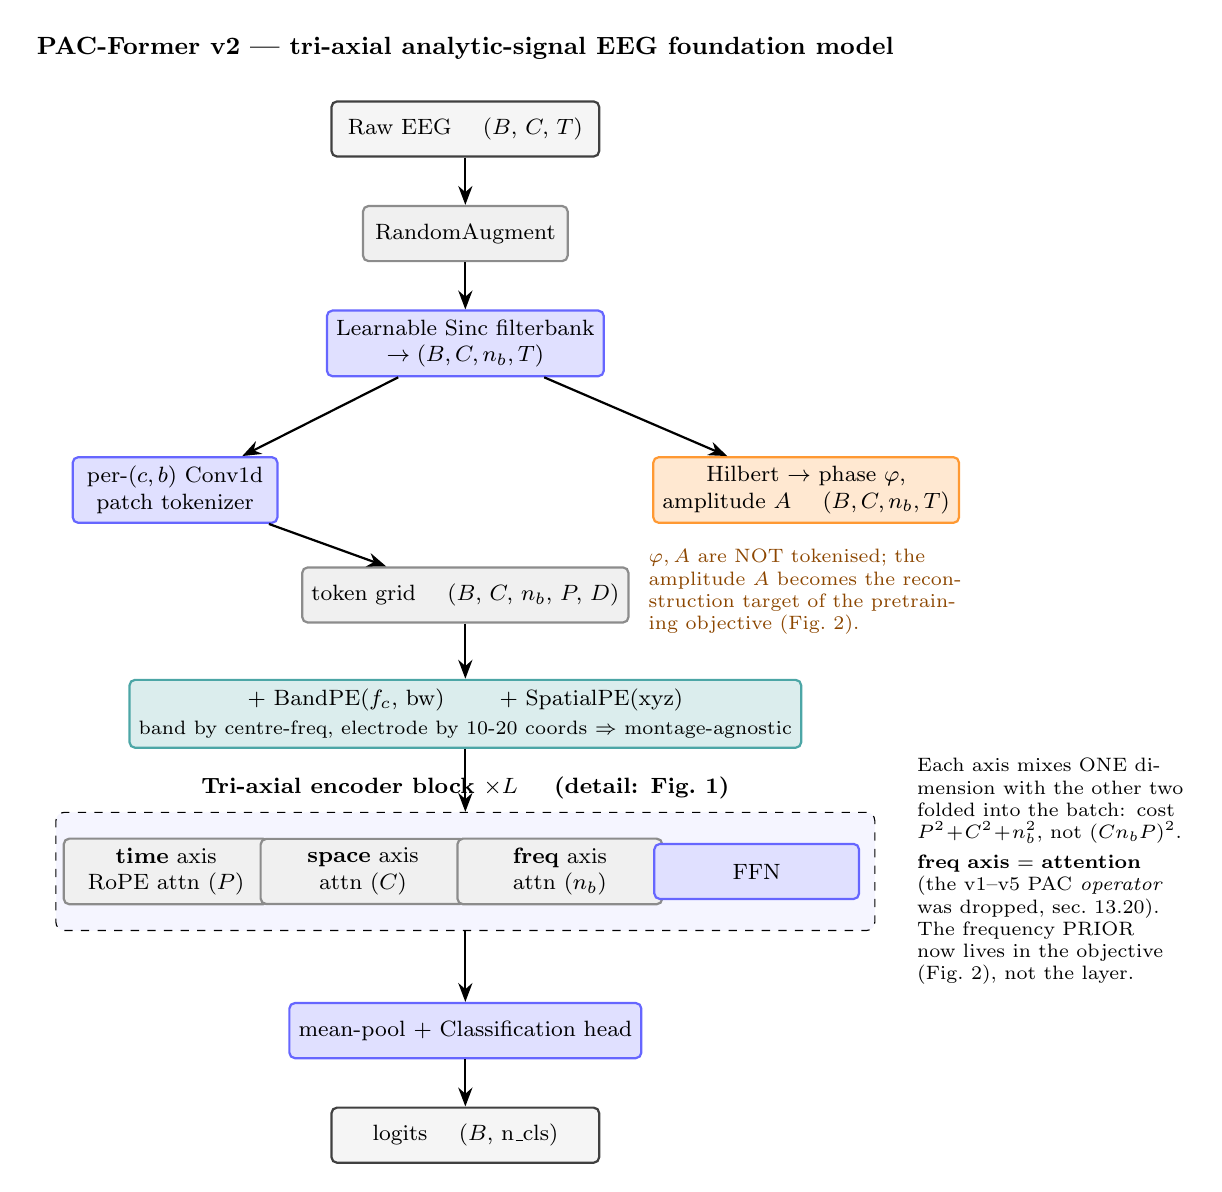
\begin{tikzpicture}[node distance=6mm]
  \node[font=\small\bfseries] (title)
        {PAC-Former v2 --- tri-axial analytic-signal EEG foundation model};

  \node[io, below=4mm of title] (raw) {Raw EEG \quad $(B,\,C,\,T)$};
  \node[op,   below=of raw]  (aug)  {RandomAugment};
  \node[learn,below=of aug]  (sinc) {Learnable Sinc filterbank\\ $\to (B,C,\nb,T)$};

  % two branches out of the band-filtered signal
  \node[learn, below left=10mm and 6mm of sinc] (tok)
        {per-$(c,b)$ Conv1d\\ patch tokenizer};
  \node[phys,  below right=10mm and 6mm of sinc] (hilb)
        {Hilbert $\to$ phase $\varphi$,\\ amplitude $A$ \quad $(B,C,\nb,T)$};

  \node[op, below=24mm of sinc] (grid) {token grid \quad $(B,\,C,\,\nb,\,P,\,D)$};

  % positional encodings (the coordinate-encoded part, sec. 13.23)
  \node[pe, below=7mm of grid] (pe)
        {$+$ BandPE$(f_c,\,\mathrm{bw})$ \qquad $+$ SpatialPE$(\mathrm{xyz})$\\[1pt]
         \scriptsize band by centre-freq, electrode by 10-20 coords $\Rightarrow$ montage-agnostic};

  % encoder
  \node[draw, dashed, rounded corners=3pt, fill=blue!4,
        minimum width=104mm, minimum height=15mm, below=8mm of pe] (enc) {};
  \node[font=\footnotesize\bfseries, above=0.4mm of enc.north]
        {Tri-axial encoder block $\times L$ \quad (detail: Fig.~1)};
  \node[op,    at={($(enc.center)+(-38mm,0)$)}] (t) {\textbf{time} axis\\ RoPE attn ($P$)};
  \node[op,    at={($(enc.center)+(-13mm,0)$)}] (s) {\textbf{space} axis\\ attn ($C$)};
  \node[op,    at={($(enc.center)+(12mm,0)$)}]  (fq){\textbf{freq} axis\\ attn ($\nb$)};
  \node[learn, at={($(enc.center)+(37mm,0)$)}]  (ffn){FFN};

  % downstream head
  \node[learn, below=9mm of enc] (head) {mean-pool $+$ Classification head};
  \node[io, below=of head] (out) {logits \quad $(B,\,\text{n\_cls})$};

  % arrows
  \draw[fl](raw)--(aug); \draw[fl](aug)--(sinc);
  \draw[fl](sinc)--(tok); \draw[fl](sinc)--(hilb);
  \draw[fl](tok)--(grid);
  \draw[fl](grid)--(pe);
  \draw[fl](pe)--(enc);
  \draw[fl](enc)--(head); \draw[fl](head)--(out);

  % note under the physiology branch: amplitude is the SSL reconstruction target
  \node[note, below=2mm of hilb, text width=40mm, orange!55!black]
        {$\varphi,A$ are NOT tokenised; the amplitude $A$ becomes the
         reconstruction target of the pretraining objective (Fig.~2).};

  \node[note, right=6mm of ffn, text width=34mm]
        {Each axis mixes ONE dimension with the other two folded into the batch:
         cost $P^2\!+\!C^2\!+\!\nb^2$, not $(C\nb P)^2$.\\[3pt]
         \textbf{freq axis $=$ attention} (the v1--v5 PAC \emph{operator} was
         dropped, sec.~13.20). The frequency PRIOR now lives in the objective
         (Fig.~2), not the layer.};
\end{tikzpicture}

% ======================================================================
% FIGURE 1 -- one tri-axial encoder block: three factorised axis mixers
% ======================================================================
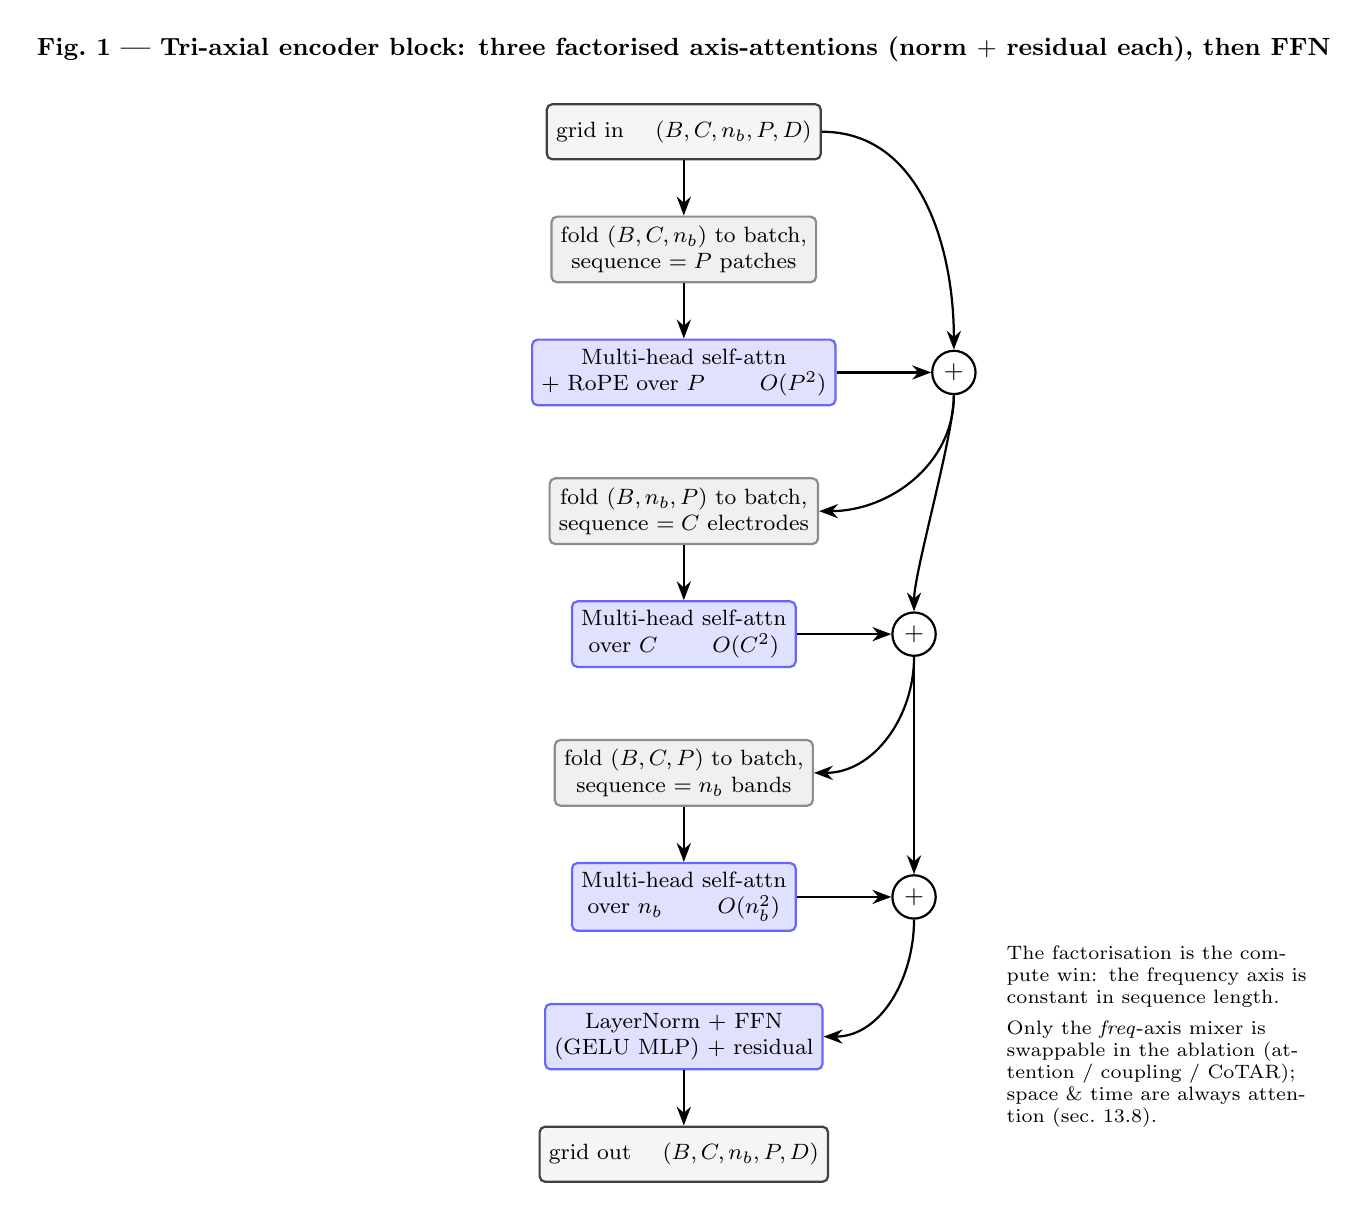
\begin{tikzpicture}[node distance=7mm]
  \node[font=\small\bfseries](title)
        {Fig.~1 --- Tri-axial encoder block: three factorised axis-attentions (norm $+$ residual each), then FFN};

  \node[io, below=4mm of title](in){grid in \quad $(B,C,\nb,P,D)$};

  % time axis
  \node[op,   below=of in](rt){fold $(B,C,\nb)$ to batch,\\ sequence $=P$ patches};
  \node[learn,below=of rt](at){Multi-head self-attn\\ $+$ RoPE over $P$ \qquad $O(P^2)$};
  \node[add,  right=12mm of at](adt){$+$};

  % space axis
  \node[op,   below=9mm of at](rs){fold $(B,\nb,P)$ to batch,\\ sequence $=C$ electrodes};
  \node[learn,below=of rs](as){Multi-head self-attn\\ over $C$ \qquad $O(C^2)$};
  \node[add,  right=12mm of as](ads){$+$};

  % freq axis
  \node[op,   below=9mm of as](rf){fold $(B,C,P)$ to batch,\\ sequence $=\nb$ bands};
  \node[learn,below=of rf](af){Multi-head self-attn\\ over $\nb$ \qquad $O(\nb^2)$};
  \node[add,  right=12mm of af](adf){$+$};

  % FFN
  \node[learn, below=9mm of af](ffn){LayerNorm $+$ FFN\\ (GELU MLP) $+$ residual};
  \node[io, below=of ffn](out){grid out \quad $(B,C,\nb,P,D)$};

  \draw[fl](in)--(rt); \draw[fl](rt)--(at); \draw[fl](at)--(adt);
  \draw[fl](in.east) to[out=0,in=90] (adt.north);
  \draw[fl](adt) to[out=-90,in=0] (rs.east);
  \draw[fl](rs)--(as); \draw[fl](as)--(ads);
  \draw[fl](adt.south) .. controls +(0,-5mm) and +(0,5mm) .. (ads.north);
  \draw[fl](ads) to[out=-90,in=0] (rf.east);
  \draw[fl](rf)--(af); \draw[fl](af)--(adf);
  \draw[fl](ads.south) .. controls +(0,-5mm) and +(0,5mm) .. (adf.north);
  \draw[fl](adf) to[out=-90,in=0] (ffn.east);
  \draw[fl](ffn)--(out);

  \node[note, right=22mm of ffn, text width=40mm]
        {The factorisation is the compute win: the frequency axis is constant in
         sequence length.\\[3pt]
         Only the \emph{freq}-axis mixer is swappable in the ablation
         (attention / coupling / CoTAR); space \& time are always attention
         (sec.~13.8).};
\end{tikzpicture}

% ======================================================================
% FIGURE 2 -- cf_mixed cross-frequency pretraining objective (THE NOVELTY)
% ======================================================================
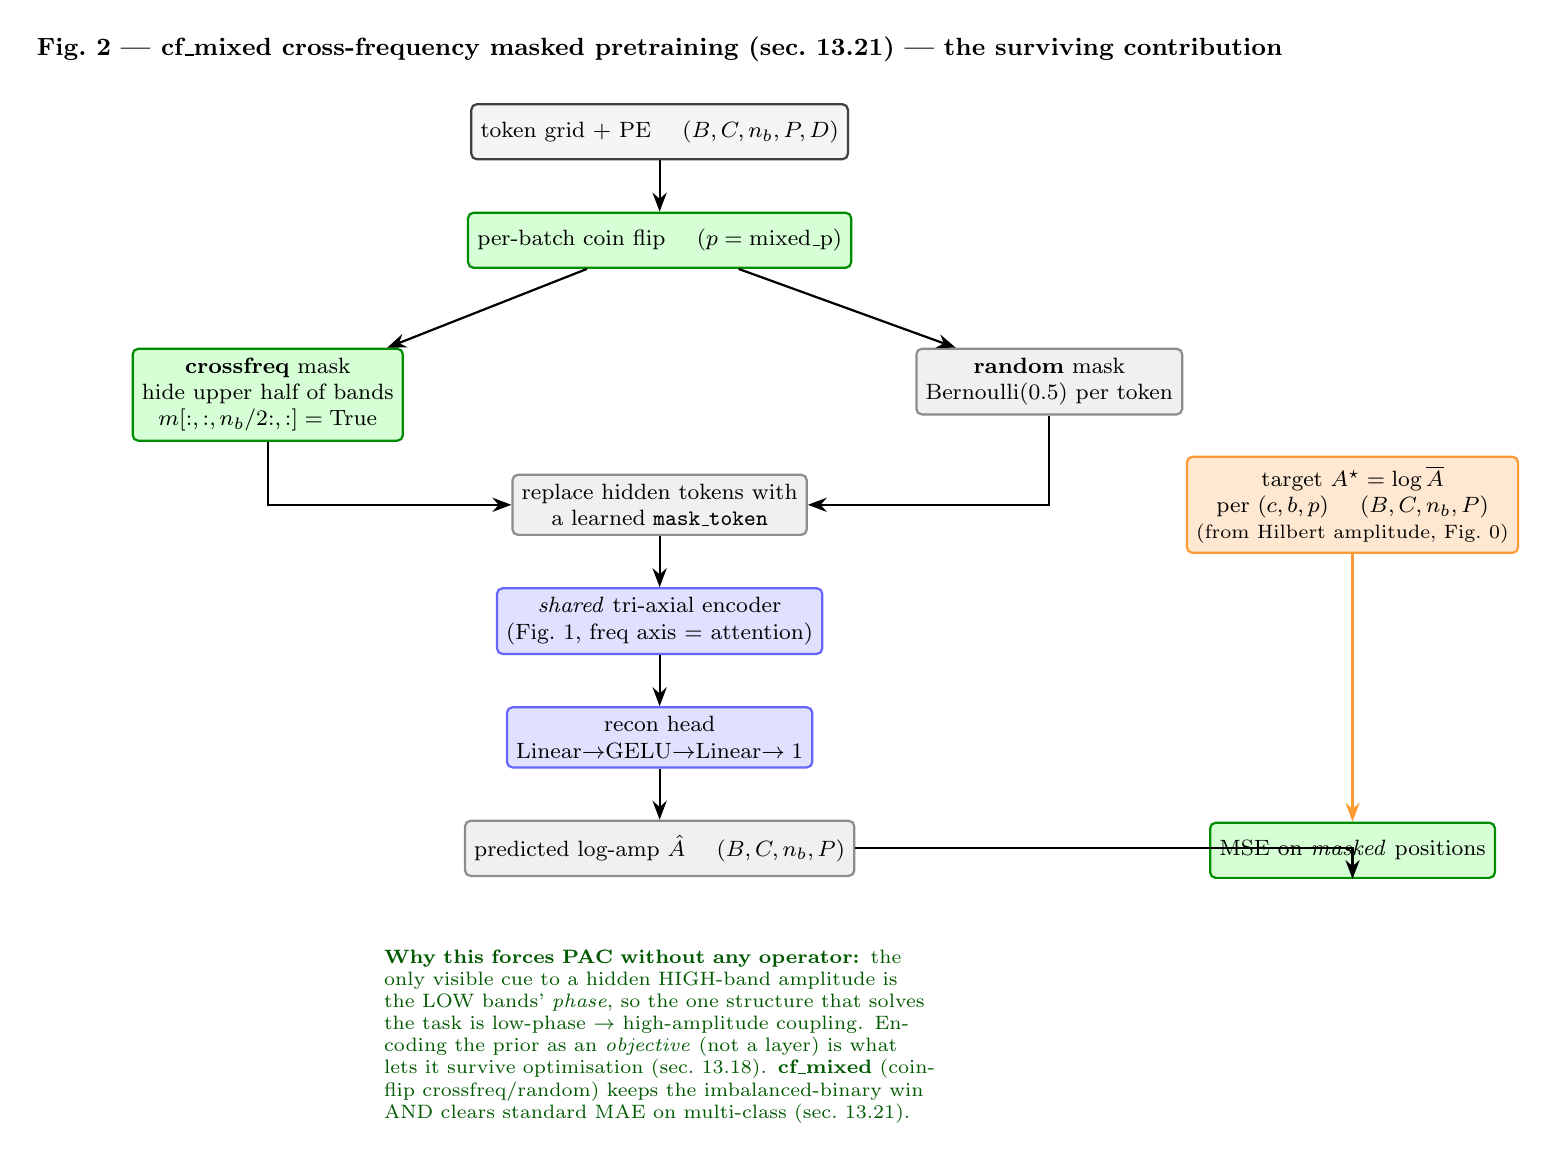
\begin{tikzpicture}[node distance=6.5mm]
  \node[font=\small\bfseries](title)
        {Fig.~2 --- \textbf{cf\_mixed} cross-frequency masked pretraining (sec.~13.21) --- the surviving contribution};

  \node[io, below=4mm of title](grid){token grid $+$ PE \quad $(B,C,\nb,P,D)$};

  % coin flip
  \node[ssl, below=of grid](flip){per-batch coin flip \quad ($p=\mathrm{mixed\_p}$)};

  % two masks
  \node[ssl, below left=10mm and 8mm of flip](cf)
        {\textbf{crossfreq} mask\\ hide upper half of bands\\ $m[:,:,\nb/2{:},:]=\mathrm{True}$};
  \node[op,  below right=10mm and 8mm of flip](rnd)
        {\textbf{random} mask\\ Bernoulli$(0.5)$ per token};

  \node[op, below=26mm of flip](masked)
        {replace hidden tokens with\\ a learned \texttt{mask\_token}};

  \node[learn, below=of masked](enc){\emph{shared} tri-axial encoder\\ (Fig.~1, freq axis $=$ attention)};
  \node[learn, below=of enc](rec){recon head\\ Linear$\to$GELU$\to$Linear$\to 1$};
  \node[op, below=of rec](pred){predicted log-amp $\hat{A}$ \quad $(B,C,\nb,P)$};

  % target column (physiology)
  \node[phys, right=48mm of masked](tgt)
        {target $A^{\star}=\log\overline{A}$\\ per $(c,b,p)$ \quad $(B,C,\nb,P)$\\
         \scriptsize (from Hilbert amplitude, Fig.~0)};
  \node[ssl, below=34mm of tgt, minimum width=34mm](lossbox)
        {MSE on \emph{masked} positions};

  \draw[fl](grid)--(flip);
  \draw[fl](flip)--(cf); \draw[fl](flip)--(rnd);
  \draw[fl](cf.south)  |- (masked.west);
  \draw[fl](rnd.south) |- (masked.east);
  \draw[fl](masked)--(enc); \draw[fl](enc)--(rec); \draw[fl](rec)--(pred);
  \draw[fl](pred.east) -| (lossbox.south);
  \draw[fl,orange!80](tgt) -- (lossbox);

  \node[note, below=8mm of pred, text width=70mm, green!35!black]
        {\textbf{Why this forces PAC without any operator:} the only visible cue
         to a hidden HIGH-band amplitude is the LOW bands' \emph{phase}, so the
         one structure that solves the task is low-phase $\to$ high-amplitude
         coupling. Encoding the prior as an \emph{objective} (not a layer) is
         what lets it survive optimisation (sec.~13.18). \textbf{cf\_mixed}
         (coin-flip crossfreq/random) keeps the imbalanced-binary win AND clears
         standard MAE on multi-class (sec.~13.21).};
\end{tikzpicture}

% ======================================================================
% FIGURE 3 -- the four architecture-ablation variants, side by side
% (sec. 13.33 defines the cells; sec. 13.37/13.39/13.40 carry the numbers)
%
% Each column is the SAME tri-axial model with exactly ONE component
% changed from the full baseline (column A). This is the from-scratch
% SUPERVISED ablation (no pretraining) used to decide which components
% earn their place before committing to the expensive pooled pretrain.
% ======================================================================
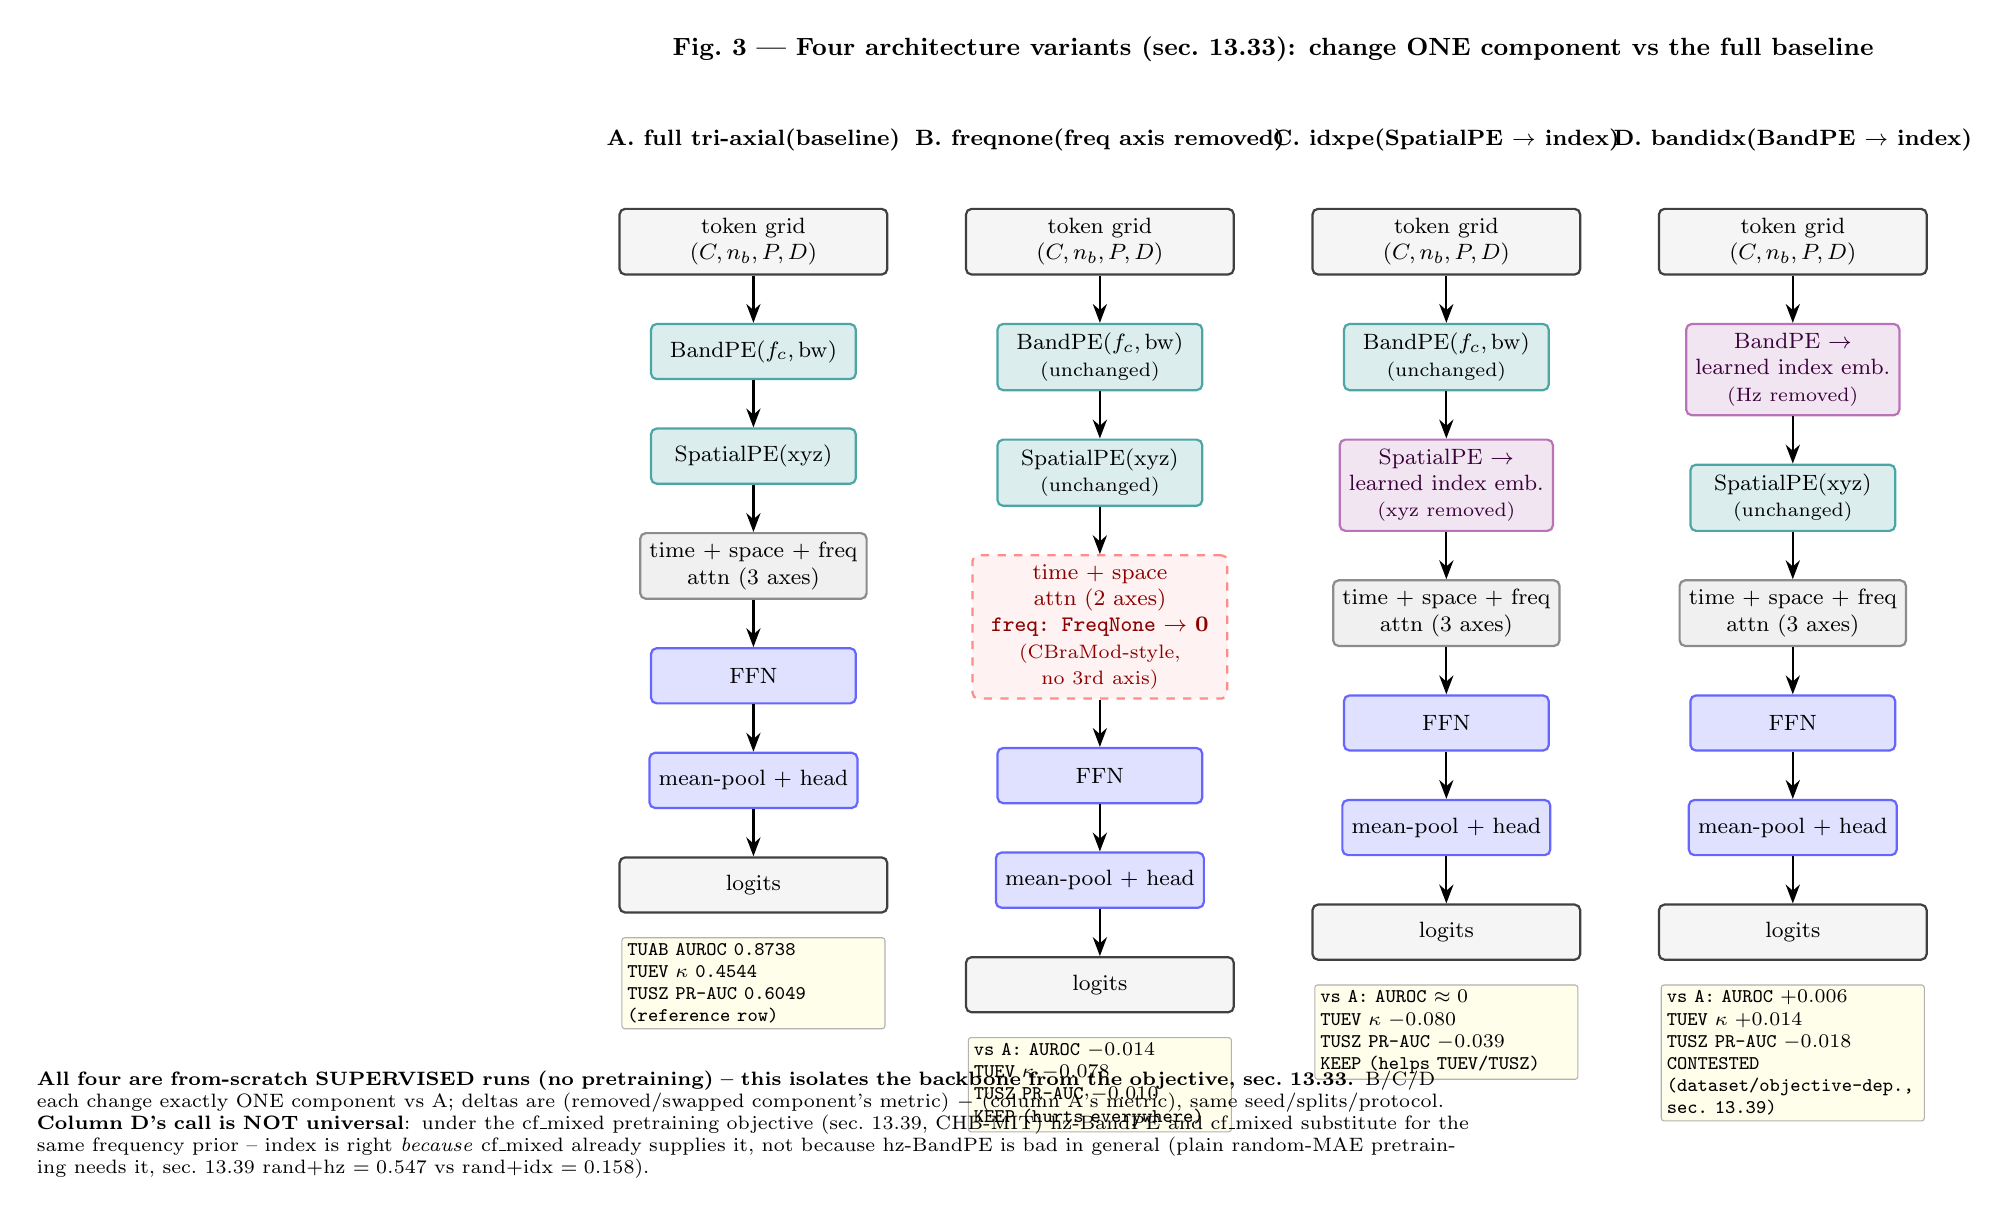
\begin{tikzpicture}[node distance=6mm]
  \node[font=\small\bfseries] (f3title)
        {Fig.~3 --- Four architecture variants (sec.~13.33): change ONE component vs the full baseline};

  % ---------------- column A: full tri-axial (baseline) -----------------
  \node[font=\footnotesize\bfseries, below=6mm of f3title, xshift=-66mm] (A-t) {A. full tri-axial\\(baseline)};
  \node[io,   below=of A-t]  (A-grid) {token grid\\$(C,\nb,P,D)$};
  \node[pe,   below=of A-grid] (A-band) {BandPE$(f_c,\mathrm{bw})$};
  \node[pe,   below=of A-band] (A-spat) {SpatialPE(xyz)};
  \node[op,   below=of A-spat] (A-axes) {time $+$ space $+$ freq\\attn (3 axes)};
  \node[learn,below=of A-axes] (A-ffn) {FFN};
  \node[learn,below=of A-ffn]  (A-head) {mean-pool $+$ head};
  \node[io,   below=of A-head] (A-out) {logits};
  \node[delta, below=3mm of A-out, text width=32mm] (A-delta)
        {TUAB AUROC 0.8738\\TUEV $\kappa$ 0.4544\\TUSZ PR-AUC 0.6049\\(reference row)};

  % ------------------- column B: freqnone -------------------------------
  \node[font=\footnotesize\bfseries, below=6mm of f3title, xshift=-22mm] (B-t) {B. freqnone\\(freq axis removed)};
  \node[io,   below=of B-t]  (B-grid) {token grid\\$(C,\nb,P,D)$};
  \node[pe,   below=of B-grid] (B-band) {BandPE$(f_c,\mathrm{bw})$\\\scriptsize(unchanged)};
  \node[pe,   below=of B-band] (B-spat) {SpatialPE(xyz)\\\scriptsize(unchanged)};
  \node[removed, below=of B-spat, text width=30mm]  (B-axes)
        {time $+$ space attn (2 axes)\\\texttt{freq: FreqNone} $\to \mathbf{0}$\\\scriptsize(CBraMod-style, no 3rd axis)};
  \node[learn,below=of B-axes] (B-ffn) {FFN};
  \node[learn,below=of B-ffn]  (B-head) {mean-pool $+$ head};
  \node[io,   below=of B-head] (B-out) {logits};
  \node[delta, below=3mm of B-out, text width=32mm] (B-delta)
        {vs A: AUROC $-0.014$\\TUEV $\kappa$ $-0.078$\\TUSZ PR-AUC $-0.010$\\\textbf{KEEP} (hurts everywhere)};

  % -------------------- column C: idxpe ----------------------------------
  \node[font=\footnotesize\bfseries, below=6mm of f3title, xshift=22mm] (C-t) {C. idxpe\\(SpatialPE $\to$ index)};
  \node[io,   below=of C-t]  (C-grid) {token grid\\$(C,\nb,P,D)$};
  \node[pe,   below=of C-grid] (C-band) {BandPE$(f_c,\mathrm{bw})$\\\scriptsize(unchanged)};
  \node[swap, below=of C-band] (C-spat) {SpatialPE $\to$\\learned index emb.\\\scriptsize(xyz removed)};
  \node[op,   below=of C-spat] (C-axes) {time $+$ space $+$ freq\\attn (3 axes)};
  \node[learn,below=of C-axes] (C-ffn) {FFN};
  \node[learn,below=of C-ffn]  (C-head) {mean-pool $+$ head};
  \node[io,   below=of C-head] (C-out) {logits};
  \node[delta, below=3mm of C-out, text width=32mm] (C-delta)
        {vs A: AUROC $\approx 0$\\TUEV $\kappa$ $-0.080$\\TUSZ PR-AUC $-0.039$\\\textbf{KEEP} (helps TUEV/TUSZ)};

  % -------------------- column D: bandidx --------------------------------
  \node[font=\footnotesize\bfseries, below=6mm of f3title, xshift=66mm] (D-t) {D. bandidx\\(BandPE $\to$ index)};
  \node[io,   below=of D-t]  (D-grid) {token grid\\$(C,\nb,P,D)$};
  \node[swap, below=of D-grid] (D-band) {BandPE $\to$\\learned index emb.\\\scriptsize(Hz removed)};
  \node[pe,   below=of D-band] (D-spat) {SpatialPE(xyz)\\\scriptsize(unchanged)};
  \node[op,   below=of D-spat] (D-axes) {time $+$ space $+$ freq\\attn (3 axes)};
  \node[learn,below=of D-axes] (D-ffn) {FFN};
  \node[learn,below=of D-ffn]  (D-head) {mean-pool $+$ head};
  \node[io,   below=of D-head] (D-out) {logits};
  \node[delta, below=3mm of D-out, text width=32mm] (D-delta)
        {vs A: AUROC $+0.006$\\TUEV $\kappa$ $+0.014$\\TUSZ PR-AUC $-0.018$\\\textbf{CONTESTED}\\(dataset/objective-dep.,\\sec.~13.39)};

  % ---- arrows within each column ----
  \foreach \col in {A,B,C,D} {
    \draw[fl](\col-grid)--(\col-band);
    \draw[fl](\col-band)--(\col-spat);
    \draw[fl](\col-spat)--(\col-axes);
  }
  \draw[fl](A-axes)--(A-ffn); \draw[fl](A-ffn)--(A-head); \draw[fl](A-head)--(A-out);
  \draw[fl](B-axes)--(B-ffn); \draw[fl](B-ffn)--(B-head); \draw[fl](B-head)--(B-out);
  \draw[fl](C-axes)--(C-ffn); \draw[fl](C-ffn)--(C-head); \draw[fl](C-head)--(C-out);
  \draw[fl](D-axes)--(D-ffn); \draw[fl](D-ffn)--(D-head); \draw[fl](D-head)--(D-out);

  \node[note, below=4mm of A-delta, text width=182mm, align=left]
        {\textbf{All four are from-scratch SUPERVISED runs (no pretraining) -- this isolates
         the backbone from the objective, sec.~13.33.} B/C/D each change exactly ONE component
         vs A; deltas are (removed/swapped component's metric) $-$ (column A's metric), same
         seed/splits/protocol. \textbf{Column D's call is NOT universal}: under the cf\_mixed
         pretraining objective (sec.~13.39, CHB-MIT) hz-BandPE and cf\_mixed substitute for the
         same frequency prior -- index is right \emph{because} cf\_mixed already supplies it,
         not because hz-BandPE is bad in general (plain random-MAE pretraining needs it,
         sec.~13.39 rand+hz $=0.547$ vs rand+idx $=0.158$).};
\end{tikzpicture}

\end{document}
